\documentclass{article}
\usepackage{float}
\usepackage{fancyhdr}
\usepackage{geometry}
\usepackage{amsmath}
\usepackage{amssymb}
\usepackage{bbm}
\usepackage{listings}
\usepackage{xcolor}
\usepackage{tikz}

\parskip = \baselineskip

\pagestyle{fancy}
\lhead{Karl Oskar Julius Olson - IE420 HW1}
\rhead{\thepage}
\renewcommand{\headrulewidth}{0.4pt}
\renewcommand{\footrulewidth}{0.4pt}

\title{IE420 - Homework 1}
\author{Karl Oskar Julius Olson}
\date{January 2020}

\begin{document}

\thispagestyle{fancy}

\section{}
\begin{align*}
	P_{ask} &= \$9.25 \\
	S &= \$318.31 \\
	K &= \$315
\end{align*}
$$N = \frac{1000}{9.25} \approx 108  \text{calls}$$
$$\text{Payoff: } (S-K)^+ = (318.31 - 315) = \$3.31, \ P\&L = \$3.13-\$9.25 = -\$5.94$$

Total loss: $P\&L \times N = -\$5.94 * 108 = -\$641.52$

Bid price on Jan 24th: $P_{bid} = \$10.30$. Rate of return is therefore: $$RoR = 100 \times \frac{P_{bid}-P_{ask}}{P_{ask}} = 100 \times \frac{\$10.30-\$9.25}{\$9.25} \approx 11.4\%$$

\section{}

\begin{align*}
	P_0 &= 313.29 \\
	S &= 318.31
\end{align*}
$$RoR = 100 \times \frac{S-P_0}{P_0} = 100 \times \frac{318.31-313-29}{313.29} \approx 1.6\%$$
Buying the \textbf{315-calls} was more profitable because they generated a rate of return of $11.4\%$ when sold at bid price on January 24th. 

\section{}

The payoff for put options is calculated as $(K-S)^+$. At the 24th of january the stock price exeeded the strike price, thus generating 0 payoff. Therefore, I would not have exercised the option.
\begin{align*}
	P_{ask}^{(0)} &= \$10.75 \\
	P_{bid}^{(T)} &= \$6.95
\end{align*}
$$RoR = 100 \times \frac{6.95-10.75}{10.75} \approx -35.3 \%$$

\section{}

\begin{figure}[H]
	\centering
	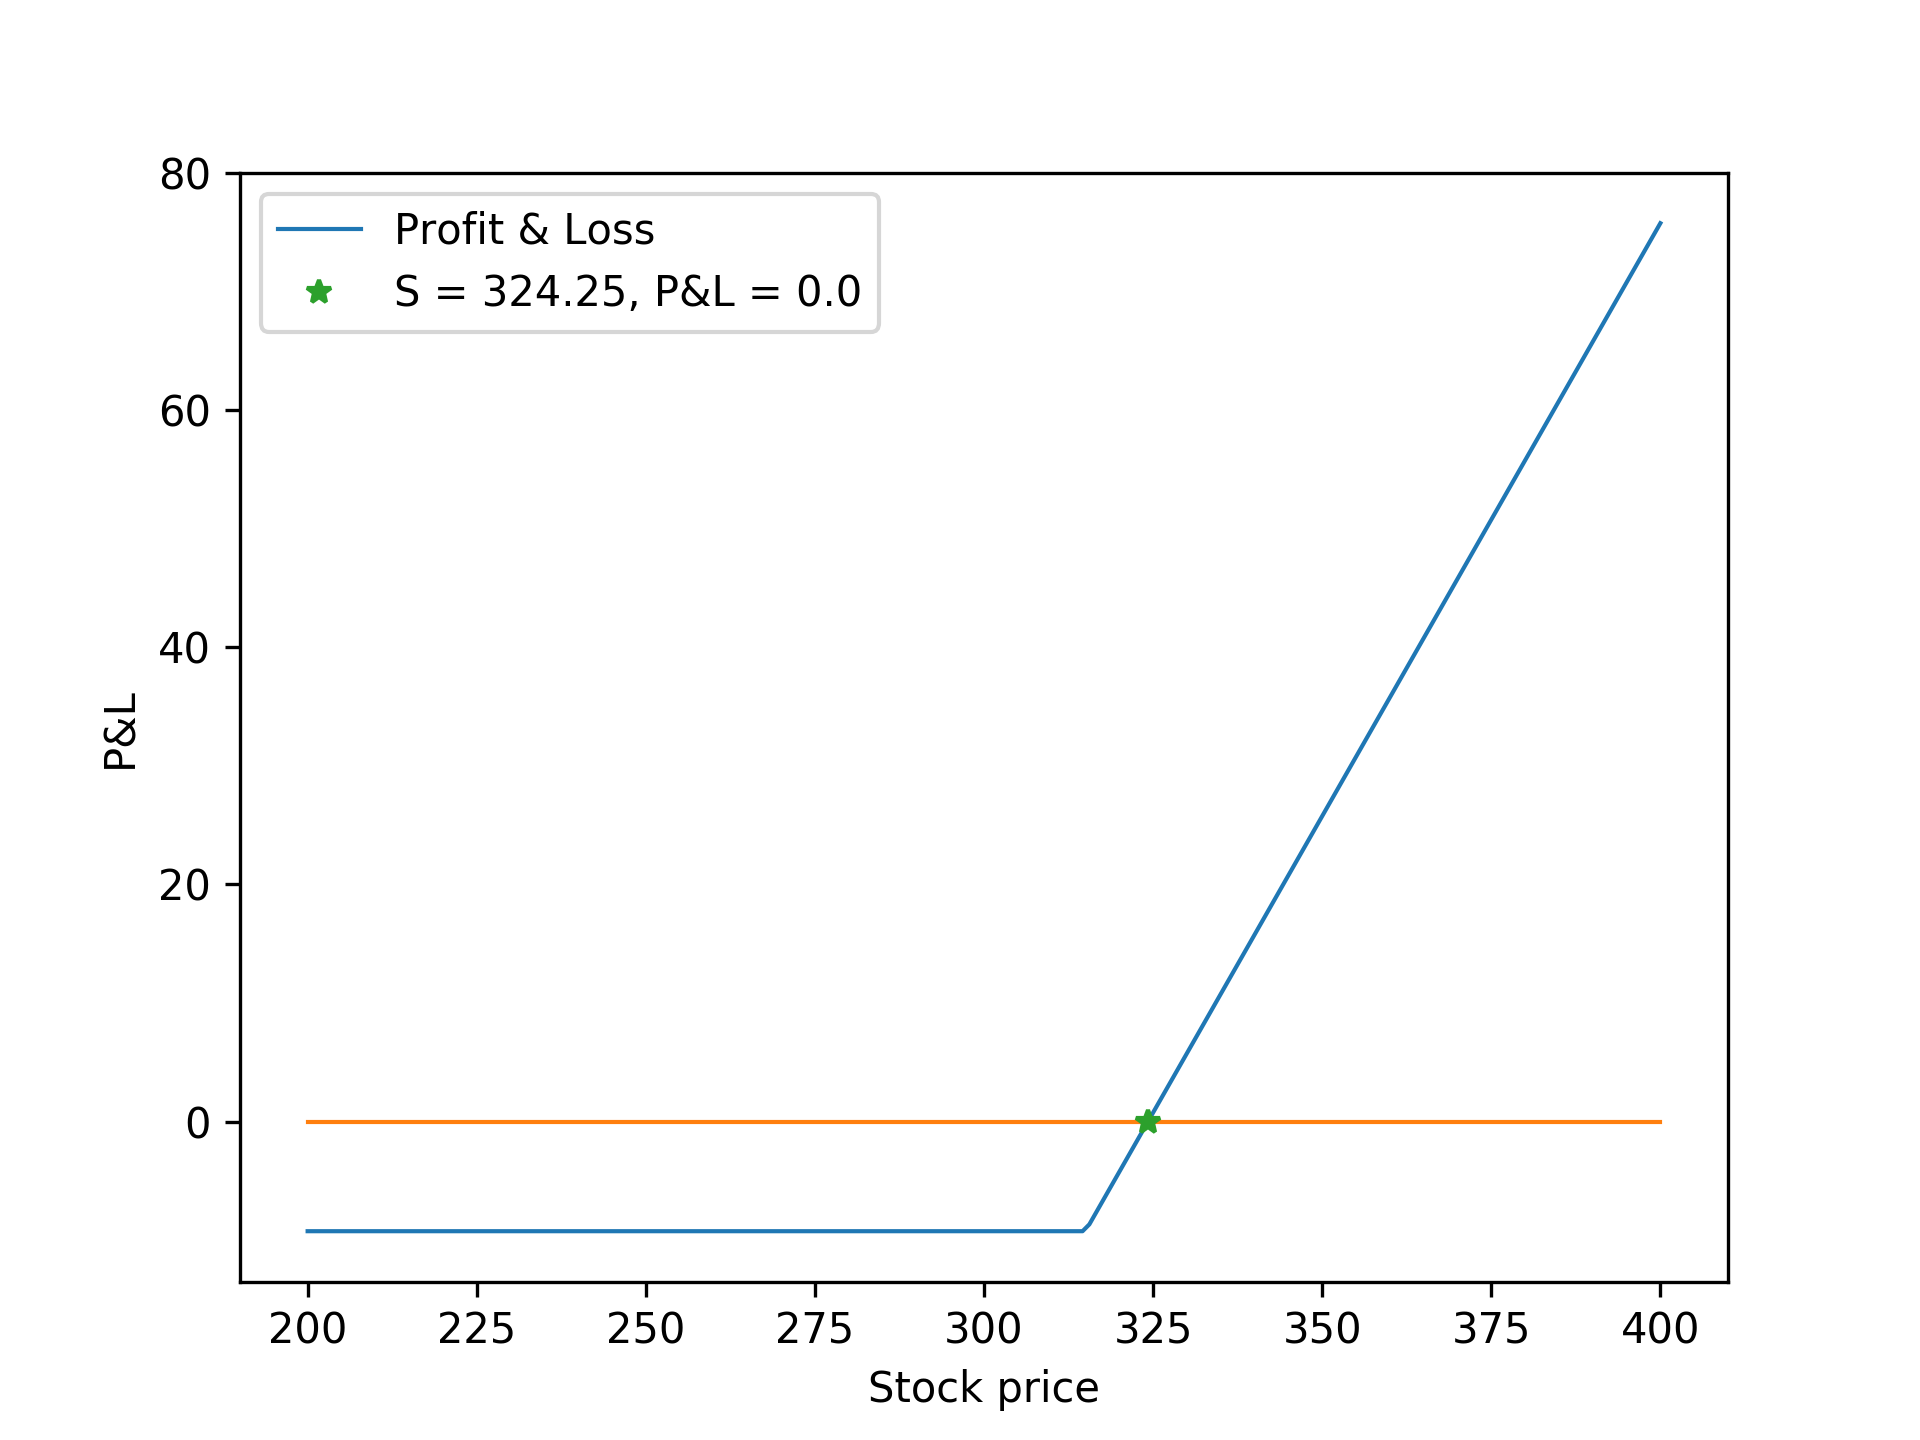
\includegraphics[width=75mm]{pl.png}
\end{figure}
The call option provides the owner with the option of buying a stock at the strike price at maturity, and not the obligation to do so. Therefore the call option owner only exercises the option if the stock price is lower than strike price. This leads to the payoff being positive, i.e $(S-K)^+ > 0$. A profit will be made if the payoff is greater than the initial price for the call option ($P_0$). The break even point (as illustrated in the plot above) is obtained when: 
$$(S-K)^+ - P_0 = 0 \implies S = K + P_0 = 315 + 9.25 = 324.25$$

\section{}

If the summer is predicted to be warmer than usual. UIUC could buy CDD (Cooling Degree Day) calls to hedge against the projected higher energy costs. A CDD follows the formula \\ 
$MAX(0, \text{daily average temp. } - 65 F)$, and therefore the value of underlying assets rises in value when the weather is warmer. Thus the call option when exercised would generate more profit the higher the average temperature was for the given contract period.

Conversly, if a very cold winter is projected, UIUC can hedge the utility costs by buying HDD (Heating Degree Day) ($MAX(0, 65F - \text{daily average temp. })$) calls. When the temperature decreases, and the utility bills increase, the value of the option's underlying asset increases and therefore can generate more profit for UIUC.


\end{document}


